% !TeX document-id = {c68f4be8-c497-43e0-82df-e9ebfbea9577}
% !TeX TXS-program:pdflatex = pdflatex -synctex=1 -interaction=nonstopmode --shell-escape %.tex
% новая команда \RNumb для вывода римских цифр
\documentclass[a4paper,12pt]{article}
\usepackage{amssymb}
\usepackage{amsmath}
\usepackage{amsthm} 
\usepackage{caption}
\usepackage{misccorr}
\usepackage[noadjust]{cite}
\usepackage{cmap} 
\usepackage[utf8]{inputenc}
\usepackage[T2A]{fontenc}
\usepackage[english, russian]{babel}
\usepackage{graphics}
\usepackage{graphicx}
\usepackage{textcomp}
\usepackage{verbatim}
\usepackage{makeidx}
\usepackage{geometry}
\usepackage{float}
\usepackage{bm}
\usepackage{esint}
\usepackage{mathtools}
\usepackage{graphicx}
\usepackage{listings}
\usepackage{courier}
\usepackage{multirow}
\usepackage{graphicx}
\usepackage[table]{xcolor}
\usepackage{color}
\usepackage[most]{tcolorbox} 
\usepackage{diagbox}

\lstset{basicstyle=\fontsize{10}{10}\selectfont,breaklines=true}

\newcommand{\specchapter}[1]{\chapter*{#1}\addcontentsline{toc}{chapter}{#1}}
\newcommand{\specsection}[1]{\section*{#1}\addcontentsline{toc}{section}{#1}}
\newcommand{\specsubsection}[1]{\subsection*{#1}\addcontentsline{toc}{subsection}{#1}}
\newcommand{\RNumb}[1]{\uppercase\expandafter{\romannumeral #1\relax}}
\newcommand{\jj}{\righthyphenmin=20 \justifying}


% геометрия
\geometry{pdftex, left = 2cm, right = 2cm, top = 2.5cm, bottom = 2.5cm}

\setcounter{tocdepth}{4} % фикс переноса 
\righthyphenmin = 2
\tolerance = 2048

\begin{document}
\thispagestyle{empty}

\noindent \begin{minipage}{0.15\textwidth}
	
\includegraphics[width=\linewidth]{b_logo}
\end{minipage}
\noindent\begin{minipage}{0.9\textwidth}\centering
	\textbf{Министерство науки и высшего образования Российской Федерации}\\
	\textbf{Федеральное государственное бюджетное образовательное учреждение высшего образования}\\
	\textbf{«Московский государственный технический университет имени Н.Э.~Баумана}\\
	\textbf{(национальный исследовательский университет)»}\\
	\textbf{(МГТУ им. Н.Э.~Баумана)}
\end{minipage}

\noindent\rule{18cm}{3pt}
\newline\newline
\noindent ФАКУЛЬТЕТ $\underline{\text{«Информатика и системы управления»}}$ \newline\newline
\noindent КАФЕДРА $\underline{\text{«Компьютерные системы и сети»}}$\newline\newline
\noindent НАПРАВЛЕНИЕ ПОДГОТОВКИ $\underline{\text{«09.03.04 Программная инженерия»}}$\newline\newline\newline\newline\newline


\begin{center}
	\noindent\begin{minipage}{1.3\textwidth}\centering
	\Large\textbf{  ОТЧЕТ }\newline
	\textbf{по лабораторной работе №4}\newline\newline
	\end{minipage}
\end{center}

\noindent\textbf{Название:} $\underline{\text{Исследование синхронных счётчиков}}$\newline\newline
\noindent\textbf{Дисциплина:} $\underline{\text{Архитектура ЭВМ}}$\newline\newline\newline\newline\newline

\begin{center}
	\begin{tabular}{ccccc}
		Студент: & $\underline{\text{ИУ7-43Б}}$ & $\underline{\text{~~~~~~~~~~~}}$ & $\underline{\text{27.04.2020}}$ & $\underline{\text{А. В. Романов}}$ \\
		 & \footnotesize группа & \footnotesize подпись & \footnotesize дата  & \footnotesize (И. О. Фамилия) \\
		  &  &  &  & \\
		Преподаватель: & \textbf{} & $\underline{\text{~~~~~~~~~~~}}$ & $\underline{\text{~~~~~~~~~~~~}}$ & $\underline{\text{А. Ю. Попов}}$ \\
		&  & \footnotesize подпись & \footnotesize дата  & \footnotesize (И. О. Фамилия) \\
	\end{tabular}
\end{center}


\begin{center}
	\vfill
	Москва~---~\the\year
~г.
\end{center}
\clearpage

\section{Цель работы} Изучение принципов построения счётчиков, овладение методом синтеза синхронных счетчиков, экспериментальная оценка динамических параметров счётчиков, изучение способов наращивания разрядности синхронных счётчиков.

\section{Исследование четырёхразрядного синхронного суммирующего счётчика с параллельным переносом на Т-триггерах.}

Схема четырёхразрядного счётчика на T-триггерах:
\begin{center}
	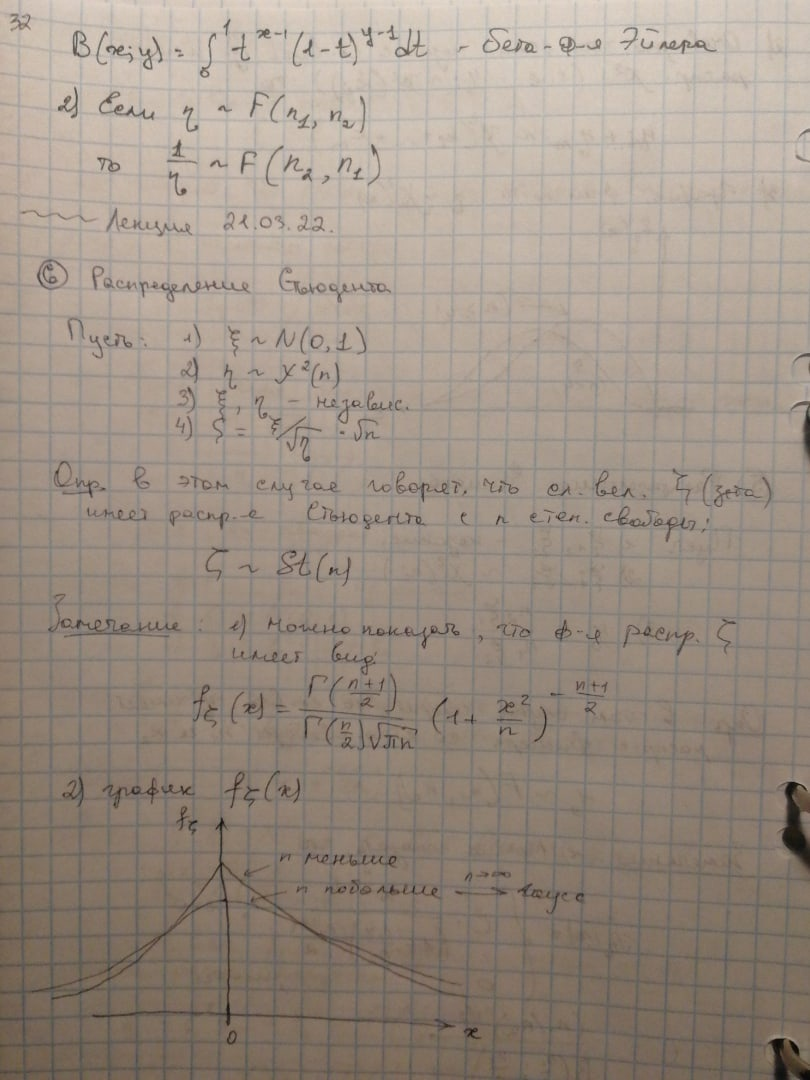
\includegraphics[scale=0.6]{../screens/1.jpg}
\end{center}

\noindent На лампочках всегда видно двоичное представление числа счётчика. При каждом замыкании-размыкании счётчик увеличивается на один. \newline

\noindent Файл: 1.ms\newline\newline

\noindent Схема с импульсным генератором и логическим анализатором сигналов
\begin{center}
	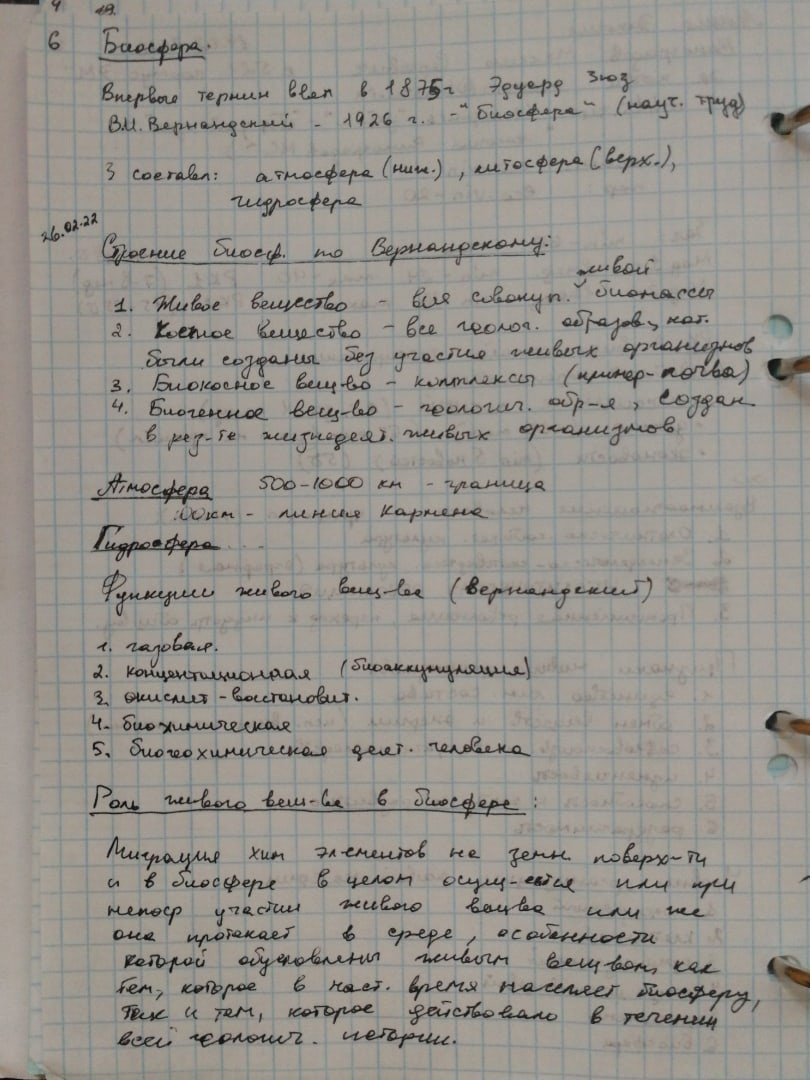
\includegraphics[scale=0.6]{../screens/2.jpg}
	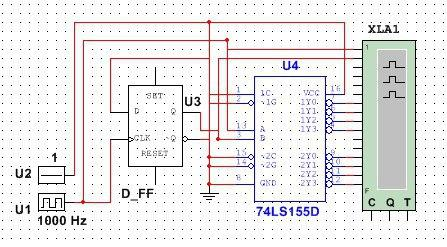
\includegraphics[scale=0.6]{../screens/2_1.jpg}
\end{center}

\noindent Собрал четырехразрядный счётчик, на выходе получаем сигналы которые равные числам от 0 до 15. Комбинируя разное кол-во триггеров, можно получать счётчики разной разрядности. \newline

\noindent Файл: 2.ms\newline

\section{Синтезировать двоично-десятичный счётчик с заданной последовательностью состояний.}

\noindent Вариант №18 (0, 1, 2, 4, 5, 6, 10, 11, 13, 14)\newline
\noindent Минимизация и таблица:
\begin{center}
	\begin{tabular}{ | l | l | l | l | l | l | l | l | l | l | l | l | l | l | l | l | p{1cm} |}
		\hline
	 	$Q_{3}$ & $Q_{2}$ & $Q_{1}$ & $Q_{0}$ & $Q_{3}*$ & $Q_{2}*$ & $Q_{1}*$ & $Q_{0}*$ & $J_{3}$ & $K_{3}$ & $J_{2}$ & $K_{2}$ & $J_{1}$ & $K_{1}$ & $J_{0}$ & $K_{0}$ \\\hline
	 	0 & 0 & 0 & 0 & 0 & 0 & 0 & 1 & 0 & $\lambda$ & 0 & $\lambda$ & 0 & $\lambda$ & 1 & $\lambda$ \\\hline
	 	0 & 0 & 0 & 1 & 0 & 0 & 1 & 0 & 0 & $\lambda$ & 0 & $\lambda$ & 1 & $\lambda$ & $\lambda$ & 1 \\\hline
	 	0 & 0 & 1 & 0 & 0 & 1 & 0 & 0 & 0 & $\lambda$ & 1 & $\lambda$ & $\lambda$ & 1 & 0 & $\lambda$ \\\hline
	 	- & - & - & - & - & - & - & - & - & - & - & - & - & - & - & - \\\hline
	 	0 & 1 & 0 & 0 & 0 & 1 & 0 & 1 & 0 & $\lambda$ & $\lambda$ & 0 & 0 & $\lambda$ & 1 & $\lambda$ \\\hline
	 	0 & 1 & 0 & 1 & 0 & 1 & 1 & 0 & 0 & $\lambda$ & $\lambda$ & 0 & 1 & $\lambda$ & $\lambda$ & 1 \\\hline
	 	0 & 1 & 1 & 0 & 1 & 0 & 1 & 0 & 1 & $\lambda$ & $\lambda$ & 1 & $\lambda$ & 0 & 0 & $\lambda$ \\\hline
	 	- & - & - & - & - & - & - & - & - & - & - & - & - & - & - & - \\\hline
	 	- & - & - & - & - & - & - & - & - & - & - & - & - & - & - & - \\\hline
	 	- & - & - & - & - & - & - & - & - & - & - & - & - & - & - & - \\\hline
	 	1 & 0 & 1 & 0 & 1 & 0 & 1 & 1 & $\lambda$ & 0 & 0 & $\lambda$ & $\lambda$ & 0 & 1 & $\lambda$ \\\hline
	 	1 & 0 & 1 & 1 & 1 & 1 & 0 & 1 & $\lambda$ & 0 & 1 & $\lambda$ & $\lambda$ & 1 & $\lambda$ & 0 \\\hline
	 	- & - & - & - & - & - & - & - & - & - & - & - & - & - & - & - \\\hline
	 	1 & 1 & 0 & 1 & 1 & 1 & 1 & 0 & $\lambda$ & 0 & $\lambda$ & 0 & 1 & $\lambda$ & $\lambda$ & 1 \\\hline
	 	1 & 1 & 1 & 0 & 0 & 0 & 0 & 0 & $\lambda$ & 1 & $\lambda$ & 1 & $\lambda$ & 1 & 0 & $\lambda$ \\\hline
	 	- & - & - & - & - & - & - & - & - & - & - & - & - & - & - & - \\
		\hline
	\end{tabular}

	""\newline
	$J_{3} = q_{2} \& q_{1}$
	
	""\newline
	\begin{tabular}{ | l | l | l | l | l | p{1cm} |}
		\hline
		\diagbox[width=5em]{$q_{3}q_{2}$}{$q_{1}q_{0}$} & 00 & 01 & 11 & 10 \\\hline
		00 & 0 & 0 & - & 0 \\\hline
		01 & 0 & 0 & \cellcolor{blue!25} - & \cellcolor{blue!25} 1 \\ \hline
		11 & - & $\lambda$ & \cellcolor{blue!25} - &  \cellcolor{blue!25} $\lambda$ \\ \hline
		10 & - & - & $\lambda$ & $\lambda$ \\ 
		\hline
	\end{tabular}

	""\newline\newline
	$K_{3} = q_{2} \& q_{1}$
	
	""\newline
	\begin{tabular}{ | l | l | l | l | l | p{1cm} |}
		\hline
		\diagbox[width=5em]{$q_{3}q_{2}$}{$q_{1}q_{0}$} & 00 & 01 & 11 & 10 \\\hline
		00 & $\lambda$ & $\lambda$ & - & $\lambda$ \\\hline
		01 & $\lambda$ & $\lambda$ & \cellcolor{blue!25} - & \cellcolor{blue!25} $\lambda$ \\ \hline
		11 & - & 0 & \cellcolor{blue!25} - &  \cellcolor{blue!25} 1  \\ \hline
		10 & - & - & 0 & 0 \\ 
		\hline
	\end{tabular}

	""\newline\newline
	$J_{2} = (\overline{q_{3}} \& q_{1})| (q_{3} \& q_{0})$
	
	""\newline
	\begin{tabular}{ | l | l | l | l | l | p{1cm} |}
		\hline
		\diagbox[width=5em]{$q_{3}q_{2}$}{$q_{1}q_{0}$} & 00 & 01 & 11 & 10 \\\hline
		00 & 0 & 0 & \cellcolor{blue!25} - & \cellcolor{blue!25} 1 \\\hline
		01 & $\lambda$ & $\lambda$ & \cellcolor{blue!25} - & \cellcolor{blue!25} $\lambda$ \\ \hline
		11 & - & \cellcolor{blue!25} $\lambda$ & \cellcolor{blue!25} - &  $\lambda$  \\ \hline
		10 & - & \cellcolor{blue!25} - & \cellcolor{blue!25} 1 & 0 \\ 
		\hline
	\end{tabular}

	""\newline\newline
	$K_{2} = q_{1}$
	
	""\newline
	\begin{tabular}{ | l | l | l | l | l | p{1cm} |}
		\hline
		\diagbox[width=5em]{$q_{3}q_{2}$}{$q_{1}q_{0}$} & 00 & 01 & 11 & 10 \\\hline
		00 & $\lambda$  & $\lambda$  & \cellcolor{blue!25} - & \cellcolor{blue!25} $\lambda$  \\\hline
		01 & 0 & 0 & \cellcolor{blue!25} - & \cellcolor{blue!25} 1 \\ \hline
		11 & - &  0 & \cellcolor{blue!25} - &  \cellcolor{blue!25} 1  \\ \hline
		10 & - & - & \cellcolor{blue!25} \cellcolor{blue!25} $\lambda$  & \cellcolor{blue!25} $\lambda$  \\ 
		\hline
	\end{tabular}

	""\newline\newline
	$J_{1} = q_{0}$
	
	""\newline
	\begin{tabular}{ | l | l | l | l | l | p{1cm} |}
		\hline
		\diagbox[width=5em]{$q_{3}q_{2}$}{$q_{1}q_{0}$} & 00 & 01 & 11 & 10 \\\hline
		00 & 0  & \cellcolor{blue!25} 1  & \cellcolor{blue!25} - & $\lambda$  \\\hline
		01 & 0  & \cellcolor{blue!25} 1  & \cellcolor{blue!25} - & $\lambda$  \\\hline
		11 & 0  & \cellcolor{blue!25} 1  & \cellcolor{blue!25} - & $\lambda$  \\\hline
		10 & -  & \cellcolor{blue!25} - & \cellcolor{blue!25} $\lambda$  & $\lambda$  \\ 
		\hline
	\end{tabular}

	\clearpage
	$K_{1} = (q_{1} \& q_{0}) | (\overline{q_{3)}} \& \overline{q_{2}}) | (q_{3} \& q_{2})$
	
	""\newline
	\begin{tabular}{ | l | l | l | l | l | p{1cm} |}
		\hline
		\diagbox[width=5em]{$q_{3}q_{2}$}{$q_{1}q_{0}$} & 00 & 01 & 11 & 10 \\\hline
		00 & \cellcolor{blue!25} $\lambda$  & \cellcolor{blue!25} $\lambda$  & \cellcolor{blue!25} - & \cellcolor{blue!25} 1  \\\hline
		01 & $\lambda$  &  $\lambda$  & \cellcolor{blue!25} - & 0  \\\hline
		11 & \cellcolor{blue!25} -  & \cellcolor{blue!25} $\lambda$  & \cellcolor{blue!25} - & \cellcolor{blue!25} 1  \\\hline
		10 & -  & - & \cellcolor{blue!25} 1  & 0  \\ 
		\hline
	\end{tabular}

	""\newline\newline
	$J_{0} = \overline{q_{1}} | (q_{3} \& \overline{q_{2)}}$
	
	""\newline
	\begin{tabular}{ | l | l | l | l | l | p{1cm} |}
		\hline
		\diagbox[width=5em]{$q_{3}q_{2}$}{$q_{1}q_{0}$} & 00 & 01 & 11 & 10 \\\hline
		00 & \cellcolor{blue!25} 1  & \cellcolor{blue!25} $\lambda$  & - & 0  \\\hline
		01 & \cellcolor{blue!25} 1  & \cellcolor{blue!25} $\lambda$  & - & 0  \\\hline
		11 & \cellcolor{blue!25} 1  & \cellcolor{blue!25} $\lambda$  & - & 0  \\\hline
		10 & \cellcolor{blue!25} -  & \cellcolor{blue!25} - & \cellcolor{blue!25} $\lambda$  & \cellcolor{blue!25} 1  \\ 
		\hline
	\end{tabular}

	""\newline\newline
	$K_{0} = \overline{q_{1}}$
	
	""\newline
	\begin{tabular}{ | l | l | l | l | l | p{1cm} |}
		\hline
		\diagbox[width=5em]{$q_{3}q_{2}$}{$q_{1}q_{0}$} & 00 & 01 & 11 & 10 \\\hline
		00 & \cellcolor{blue!25} $\lambda$  & \cellcolor{blue!25} 1  & - & $\lambda$  \\\hline
		01 & \cellcolor{blue!25} $\lambda$  & \cellcolor{blue!25} 1  & - & $\lambda$  \\\hline
		11 & \cellcolor{blue!25} -  & \cellcolor{blue!25} 1 & - & $\lambda$  \\\hline
		10 & \cellcolor{blue!25} -  & \cellcolor{blue!25} - & 0  & $\lambda$  \\ 
		\hline
	\end{tabular}

\end{center}
	""\newline\newline
	Схема на логических элементах и $JK$-тригерах:
	
\begin{center}
	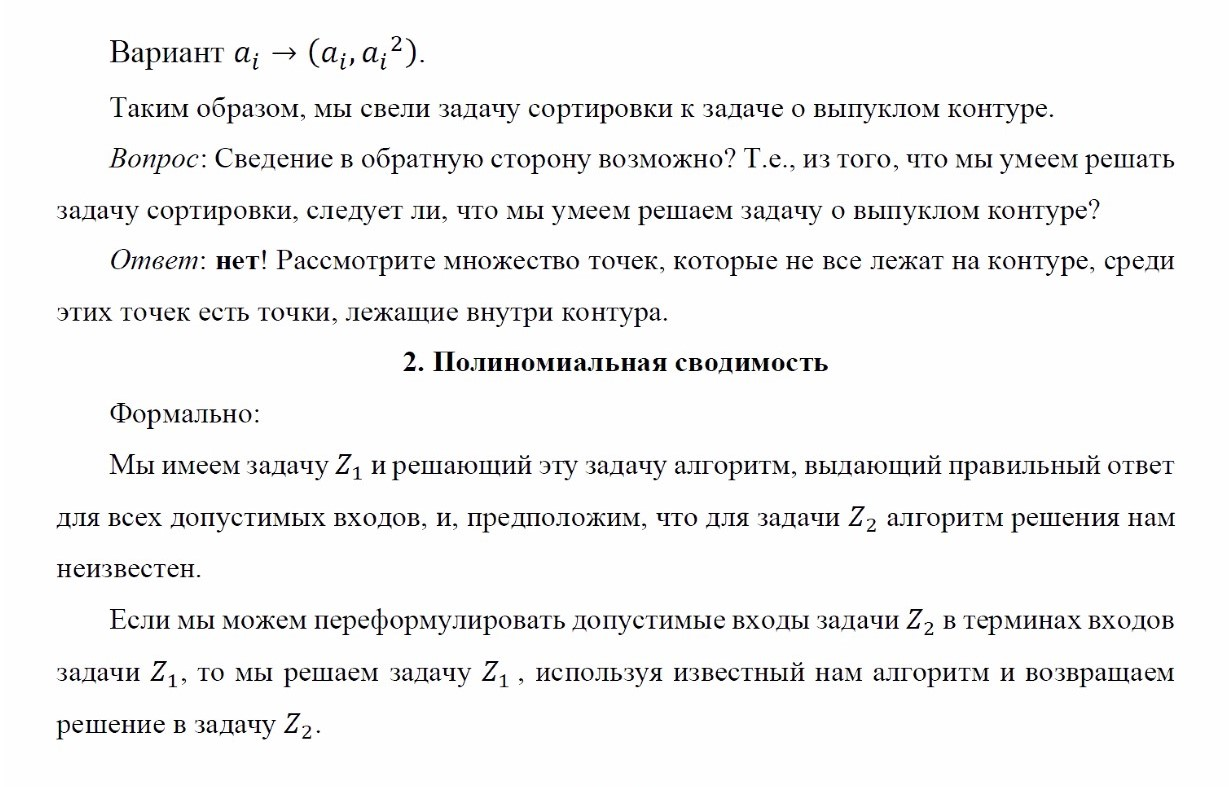
\includegraphics[scale=0.58]{../screens/3.jpg}
\end{center}

\noindent Файл: 3.ms

\section{Собрать десятичный счётчик, используя элементную базу приложения Multisim или учебного макета}
\noindent Минимизация и таблица:
\begin{center}
	\begin{tabular}{ | l | l | l | l | l | l | l | l | l | l | l | l | l | l | l | l | p{1cm} |}
		\hline
		$Q_{3}$ & $Q_{2}$ & $Q_{1}$ & $Q_{0}$ & $Q_{3}*$ & $Q_{2}*$ & $Q_{1}*$ & $Q_{0}*$ & $J_{3}$ & $K_{3}$ & $J_{2}$ & $K_{2}$ & $J_{1}$ & $K_{1}$ & $J_{0}$ & $K_{0}$ \\\hline
		0 & 0 & 0 & 0 & 0 & 0 & 0 & 1 & 0 & $\alpha$ & 0 & $\alpha$ & 0 & $\alpha$ & 1 & $\alpha$ \\\hline
		0 & 0 & 0 & 1 & 0 & 0 & 1 & 0 & 0 & $\alpha$ & 0 & $\alpha$ & 1 & $\alpha$ & $\alpha$ & 1 \\\hline
		0 & 0 & 1 & 0 & 0 & 0 & 1 & 1 & 0 & $\alpha$ & 0 & $\alpha$ & $\alpha$ & 0 & 1 & $\alpha$ \\\hline
		0 & 0 & 1 & 1 & 0 & 1 & 0 & 0 & 0 & $\alpha$ & 1 & $\alpha$ & $\alpha$ & 1 & $\alpha$ & 1 \\\hline
		0 & 1 & 0 & 0 & 0 & 1 & 0 & 1 & 0 & $\alpha$ & $\alpha$ & 0 & 0 & $\alpha$ & 1 & $\alpha$ \\\hline
		0 & 1 & 0 & 1 & 0 & 1 & 1 & 0 & 0 & $\alpha$ & $\alpha$ & 0 & 1 & $\alpha$ & $\alpha$ & 1 \\\hline
		0 & 1 & 1 & 0 & 0 & 1 & 1 & 1 & 0 & $\alpha$ & $\alpha$ & 0 & $\alpha$ & 0 & 1 & $\alpha$ \\\hline
		0 & 1 & 1 & 1 & 1 & 0 & 0 & 0 & 1 & $\alpha$ & $\alpha$ & 1 & $\alpha$ & 1 & $\alpha$ & 1 \\\hline
		1 & 0 & 0 & 0 & 1 & 0 & 0 & 1 & $\alpha$ & 0 & 0 & $\alpha$ & 0 & $\alpha$ & 1 & $\alpha$ \\\hline
		1 & 0 & 0 & 1 & 0 & 0 & 0 & 0 & $\alpha$ & 1 & 0 & $\alpha$ & 0 & $\alpha$ & $\alpha$ & 1 \\\hline
		- & - & - & - & - & - & - & - & - & - & - & - & - & - & - & - \\\hline
		- & - & - & - & - & - & - & - & - & - & - & - & - & - & - & - \\\hline
		- & - & - & - & - & - & - & - & - & - & - & - & - & - & - & - \\\hline
		- & - & - & - & - & - & - & - & - & - & - & - & - & - & - & - \\\hline
		- & - & - & - & - & - & - & - & - & - & - & - & - & - & - & - \\\hline
		- & - & - & - & - & - & - & - & - & - & - & - & - & - & - & - \\
		\hline
	\end{tabular}

	""\newline\newline
	$J_{3} = q_{0} \& q_{1} \& q_{2}$
	
	""\newline
	\begin{tabular}{ | l | l | l | l | l | p{1cm} |}
		\hline
		\diagbox[width=5em]{$q_{3}q_{2}$}{$q_{1}q_{0}$} & 00 & 01 & 11 & 10 \\\hline
		00 & 0 & 0  & 0 & 0  \\\hline
		01 & 0 & 0  & \cellcolor{blue!25} 1 & 0  \\\hline
		11 & - & -  & \cellcolor{blue!25} - & -  \\\hline
		10 & $\alpha$ & $\alpha$  & - & -  \\
		\hline
	\end{tabular}

	""\newline\newline
	$K_{3} = q_{0}$
	
	""\newline
	\begin{tabular}{ | l | l | l | l | l | p{1cm} |}
		\hline
		\diagbox[width=5em]{$q_{3}q_{2}$}{$q_{1}q_{0}$} & 00 & 01 & 11 & 10 \\\hline
		00 & $\alpha$ & \cellcolor{blue!25} $\alpha$  & \cellcolor{blue!25} $\alpha$ & $\alpha$  \\\hline
		01 & $\alpha$ & \cellcolor{blue!25} $\alpha$  & \cellcolor{blue!25} $\alpha$ & $\alpha$  \\\hline
		11 & - & \cellcolor{blue!25} -  & \cellcolor{blue!25} - & -  \\\hline
		10 & 0 & \cellcolor{blue!25} 1  & \cellcolor{blue!25} - & -  \\
		\hline
	\end{tabular}

	\clearpage
	$J_{2} = q_{0} \& q_{1}$
	
	""\newline
	\begin{tabular}{ | l | l | l | l | l | p{1cm} |}
		\hline
		\diagbox[width=5em]{$q_{3}q_{2}$}{$q_{1}q_{0}$} & 00 & 01 & 11 & 10 \\\hline
		00 & 0 & 0  & \cellcolor{blue!25} 1 & 0  \\\hline
		01 & $\alpha$ & $\alpha$ & \cellcolor{blue!25} $\alpha$ & $\alpha$  \\\hline
		11 & - & -  & \cellcolor{blue!25} - & -  \\\hline
		10 & 0 & 0  & \cellcolor{blue!25} - & -  \\
		\hline
	\end{tabular}

	""\newline\newline
	$K_{2} = q_{0} \& q_{1}$
	
	""\newline
	\begin{tabular}{ | l | l | l | l | l | p{1cm} |}
		\hline
		\diagbox[width=5em]{$q_{3}q_{2}$}{$q_{1}q_{0}$} & 00 & 01 & 11 & 10 \\\hline
		00 & $\alpha$ & $\alpha$  & \cellcolor{blue!25} $\alpha$ & $\alpha$  \\\hline
		01 & 0 & 0  & \cellcolor{blue!25} 1 & 0  \\\hline
		11 & - & -  & \cellcolor{blue!25} - & -  \\\hline
		10 & $\alpha$ & $\alpha$ & \cellcolor{blue!25} - & -  \\
		\hline
	\end{tabular}

	""\newline\newline
	$J_{1} = q_{0} \& \overline{q_{3}}$
	
	""\newline
	\begin{tabular}{ | l | l | l | l | l | p{1cm} |}
		\hline
		\diagbox[width=5em]{$q_{3}q_{2}$}{$q_{1}q_{0}$} & 00 & 01 & 11 & 10 \\\hline
		00 & 0 & \cellcolor{blue!25} 1  & \cellcolor{blue!25} $\alpha$ & $\alpha$  \\\hline
		01 & 0 & \cellcolor{blue!25} 1  & \cellcolor{blue!25} $\alpha$ & $\alpha$  \\\hline
		11 & - & -  & - & -  \\\hline
		10 & 0 & 0  & - & -  \\
		\hline
	\end{tabular}

	""\newline\newline
	$K_{1} = q_{0}$
	
	""\newline
	\begin{tabular}{ | l | l | l | l | l | p{1cm} |}
		\hline
		\diagbox[width=5em]{$q_{3}q_{2}$}{$q_{1}q_{0}$} & 00 & 01 & 11 & 10 \\\hline
		00 & $\alpha$ & \cellcolor{blue!25} $\alpha$  & \cellcolor{blue!25} 1 & 0  \\\hline
		01 & $\alpha$ & \cellcolor{blue!25} $\alpha$  & \cellcolor{blue!25} 1 & 0  \\\hline
		11 & - & \cellcolor{blue!25} -  & \cellcolor{blue!25} - & -  \\\hline
		10 & $\alpha$ & \cellcolor{blue!25} $\alpha$ & \cellcolor{blue!25} - & -  \\
		\hline
	\end{tabular}

	""\newline\newline
	$J_{0} = 1$
	
	""\newline
	\begin{tabular}{ | l | l | l | l | l | p{1cm} |}
		\hline
		\diagbox[width=5em]{$q_{3}q_{2}$}{$q_{1}q_{0}$} & 00 & 01 & 11 & 10 \\\hline
		00 & \cellcolor{blue!25} 1 & \cellcolor{blue!25} $\alpha$ & \cellcolor{blue!25} $\alpha$ & \cellcolor{blue!25} 1  \\\hline
		01 & \cellcolor{blue!25} 1 & \cellcolor{blue!25} $\alpha$ & \cellcolor{blue!25} $\alpha$ & \cellcolor{blue!25} 1  \\\hline
		11 & \cellcolor{blue!25} - & \cellcolor{blue!25} -  & \cellcolor{blue!25} - & \cellcolor{blue!25} -  \\\hline
		10 & \cellcolor{blue!25} 1 & \cellcolor{blue!25} $\alpha$  & \cellcolor{blue!25} - & \cellcolor{blue!25} -  \\
		\hline
	\end{tabular}

	\clearpage
	$K_{0} = 1$
	
	""\newline
	\begin{tabular}{ | l | l | l | l | l | p{1cm} |}
		\hline
		\diagbox[width=5em]{$q_{3}q_{2}$}{$q_{1}q_{0}$} & 00 & 01 & 11 & 10 \\\hline
		00 & \cellcolor{blue!25} $\alpha$ & \cellcolor{blue!25} 1 & \cellcolor{blue!25} 1 & \cellcolor{blue!25} $\alpha$  \\\hline
		01 & \cellcolor{blue!25} $\alpha$ & \cellcolor{blue!25} 1 & \cellcolor{blue!25} 1 & \cellcolor{blue!25} $\alpha$  \\\hline
		11 & \cellcolor{blue!25}- & \cellcolor{blue!25}-  & \cellcolor{blue!25} - & \cellcolor{blue!25} -  \\\hline
		10 & \cellcolor{blue!25} $\alpha$ & \cellcolor{blue!25}1  & \cellcolor{blue!25} - & \cellcolor{blue!25} -  \\
		\hline
	\end{tabular}
\end{center}

""\newline\newline
\noindent Схема:
\begin{center}
	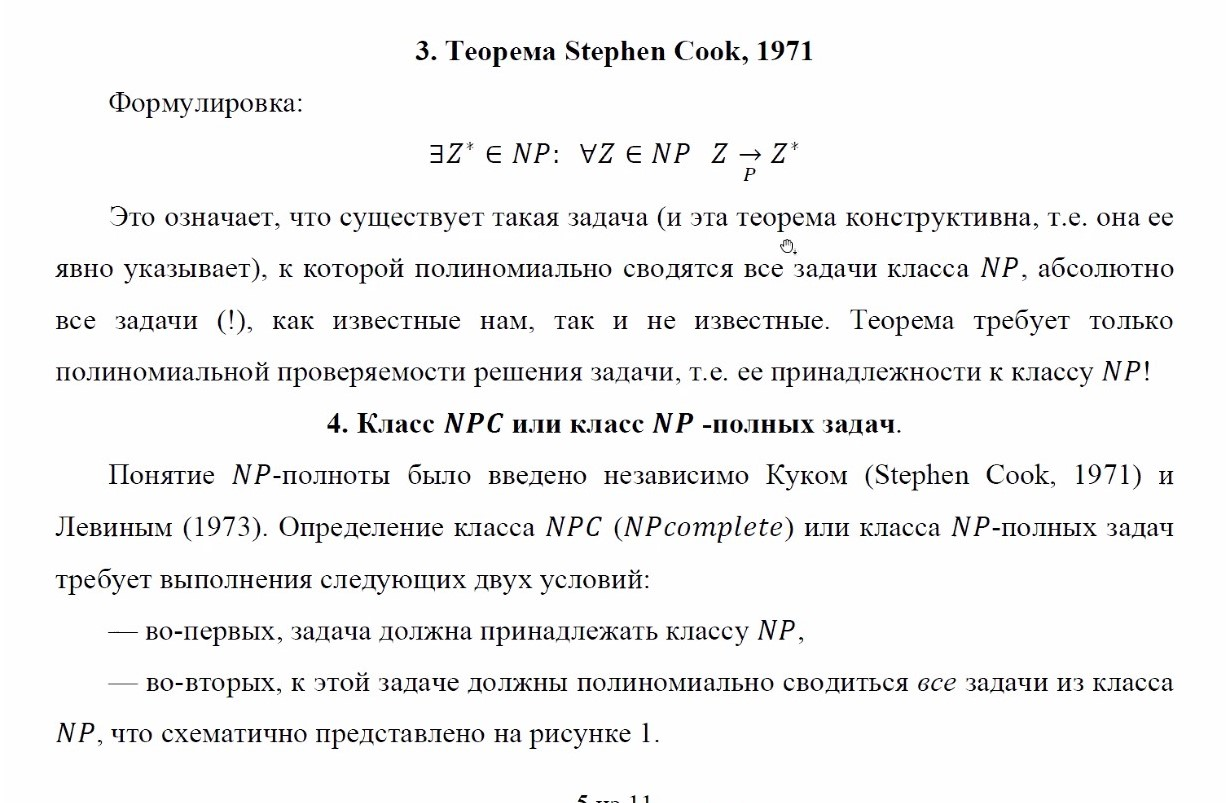
\includegraphics[scale=0.8]{../screens/4.jpg}
\end{center}

""\newline
\noindent Полученая схема - счётчик в двоично-десятичной СС. По данной схеме так же можно строить счётчики произвольного порядка.\newline

\noindent Файл: 4.ms\newline

\section{Исследование четырёхразрядного синхронного суммирующего счётчика с параллельным переносом.}
 
\begin{center}
	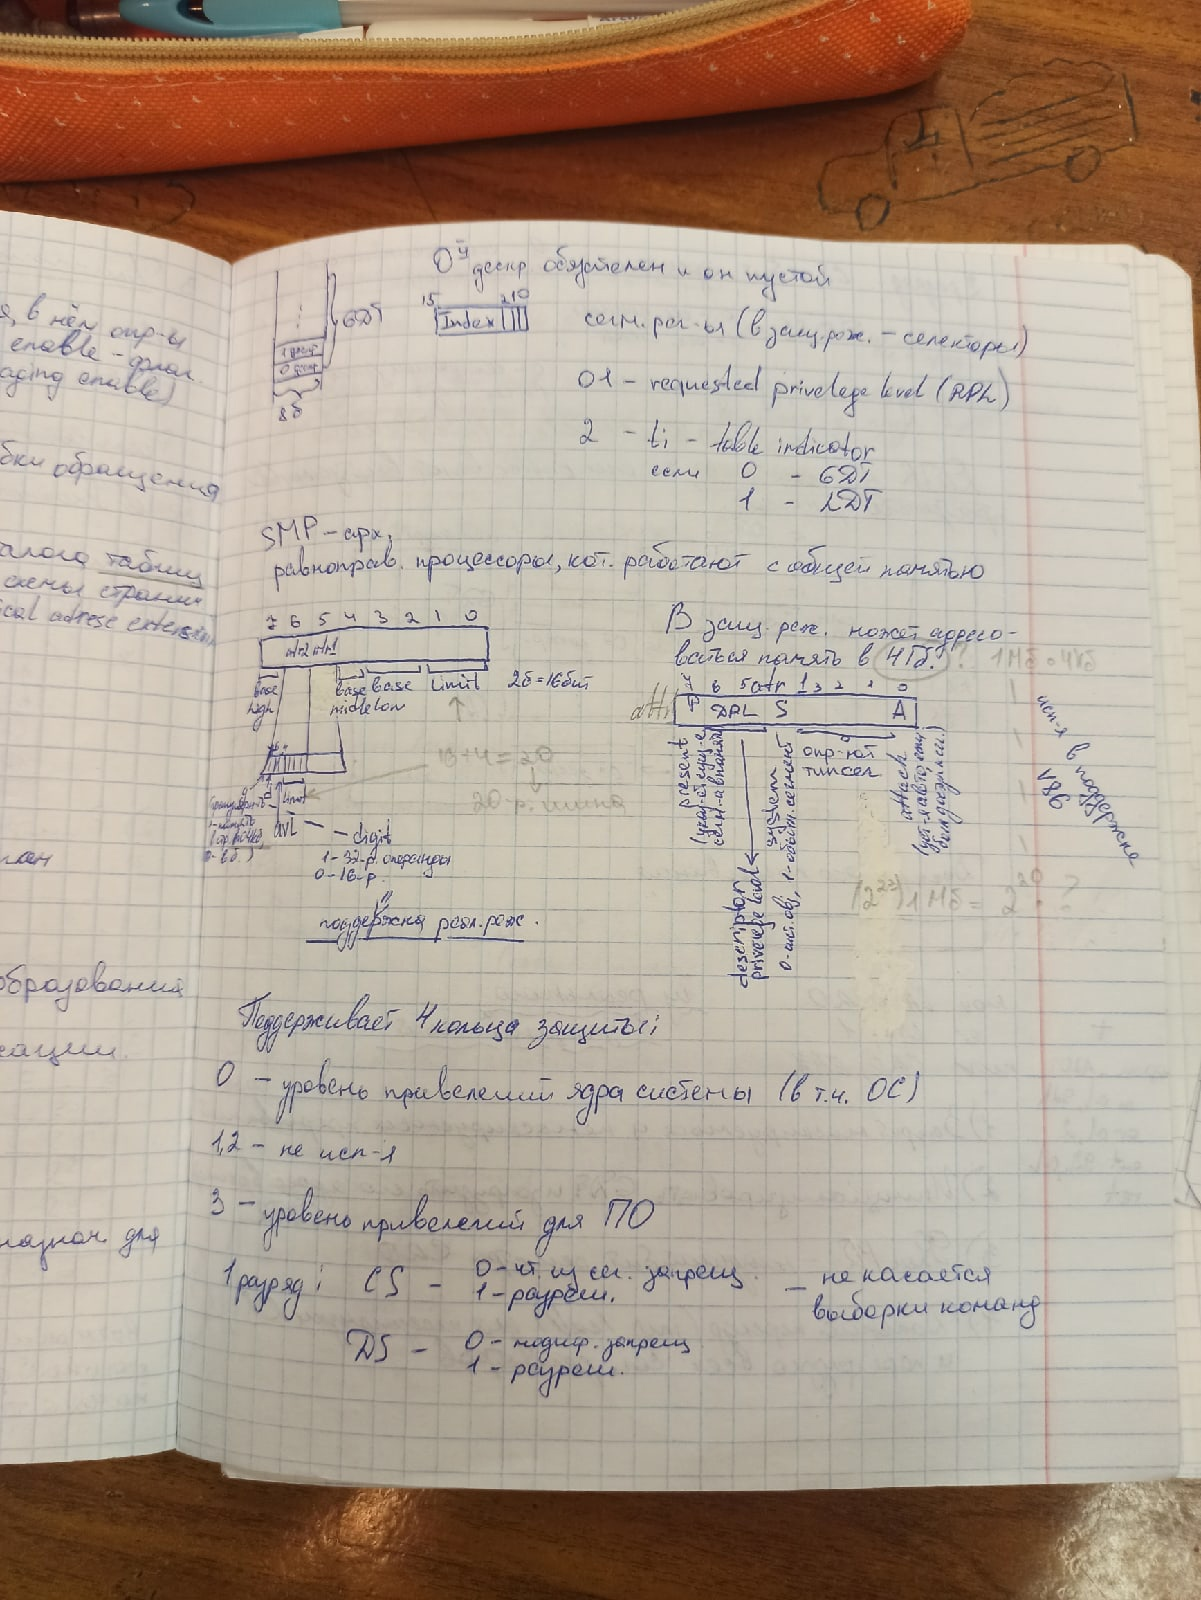
\includegraphics[scale=0.72]{../screens/5.jpg}
	
	""\newline
	
	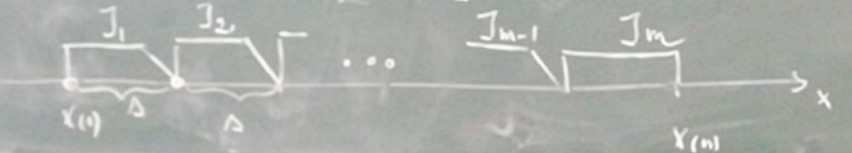
\includegraphics[scale=0.72]{../screens/5_1.jpg}
	
	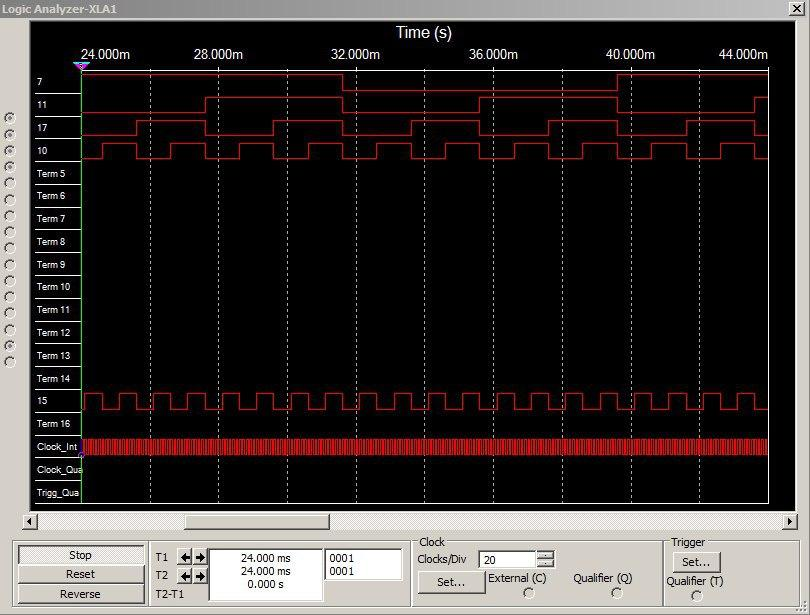
\includegraphics[scale=0.75]{../screens/5_2.jpg}
\end{center}

""\newline\newline
\noindent Получили счётчик в 16CC, обнуляется когда доходит до F.\newline

\noindent Файлы: 5.ms и 6.ms\newline

\section{Исследование четырёхразрядного синхронного суммирующего счётчика с параллельным переносом ИС К555ИЕ9}

Одиночные импульсы:
\begin{center}
	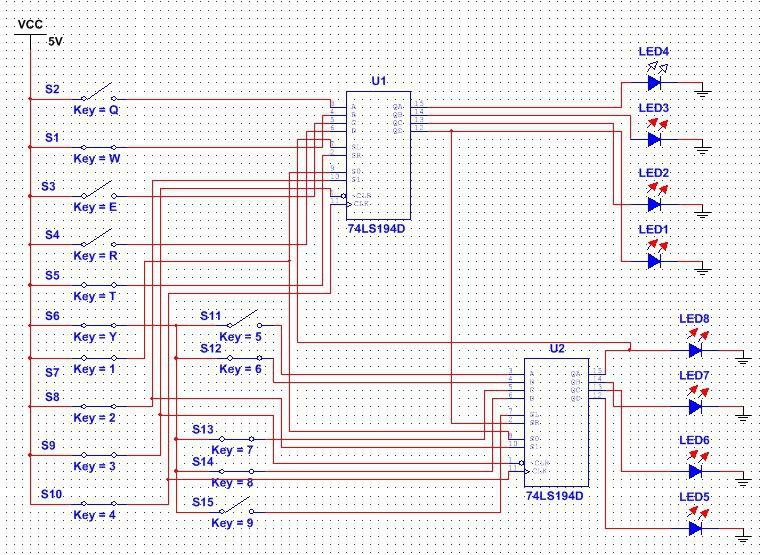
\includegraphics[scale=0.75]{../screens/6.jpg}
\end{center}

От импульсов генератора:

\begin{center}
	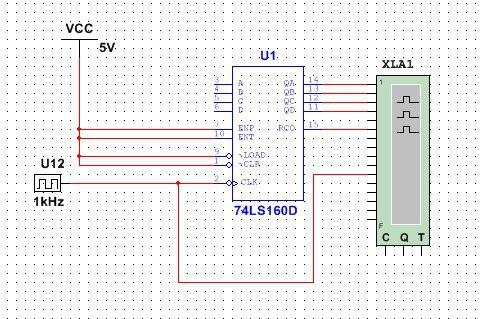
\includegraphics[scale=1]{../screens/6_1.jpg}
	
	""\newline\newline
	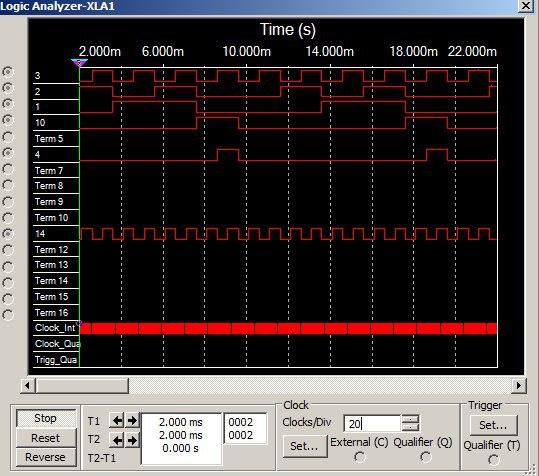
\includegraphics[scale=0.9]{../screens/6_2.jpg}
\end{center}

""\newline
\noindent Файлы: 7.ms и 8.ms

\section{Исследование схем наращивания разрядности счётчиков ИЕ9 до четырех секций с последовательным переносом между секциями и по структуре «быстрого» счёта.}

\begin{center}
	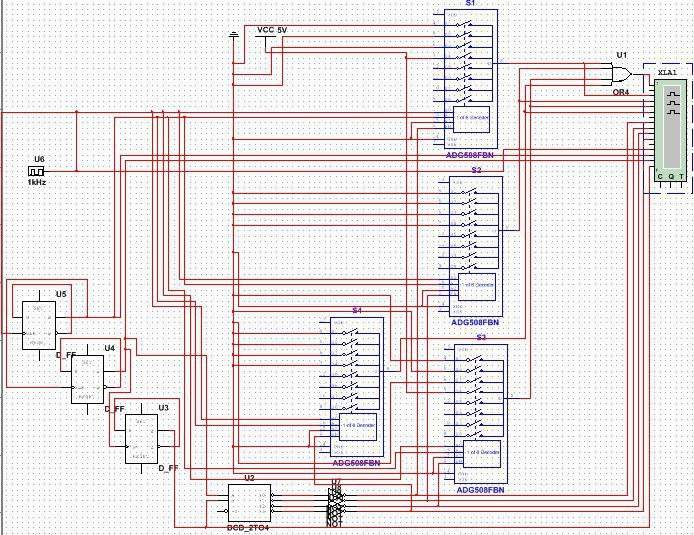
\includegraphics[scale=0.6]{../screens/7.jpg}
\end{center}


\noindent Получаем многоразрядный десятичный счётчик. Итоговое число нужно читать справа налево.\newline

\noindent Файл: 9.ms

\section{Вывод}

\noindent При выполнении этой лабораторной работы я изучил принципы построения счётчиков, способы наращивания разрядности синхронных счётчиков, овладел методом синтеза синхронных счетчиков

\section{Контрольные вопросы}

\noindent\textbf{1.} Что называется счётчиком?\newline

\noindent\textbf{Счётчик} -- это операционный узел ЭВМ, предназначенный для выполнения счёта, кодирования в определённой системе счисления и хранения числа сигналов импульсного типа, поступающих на счётный вход.
\newline

\clearpage
\noindent\textbf{2.} Что называется коэффициентом пересчёта? \newline

\noindent\textbf{Коэффициент пересчёта} -- число входных сигналов, которое возвращает схему в начальное состояние, в качестве которого может быть взято любое её состояние.
\newline

\noindent\textbf{3.} Перечислить основные классификационные признаки счётчиков.\newline

\noindent \textbf{По значению модуля счёта}:\newline

\noindent - Двоичные счётчики ($M = 2^n,$ $n$ - кол-во двоичных разрядов)

\noindent - Двоичное кодированные счётчики

\noindent - Счётчики с одинарным кодированием (состояние представлено местом расположения едиснвтенной единицы)\newline

\noindent Помимо этих, существуют счётчики классификации по направлению счёта, по способу организации межразрядных связей, по порядку изменения состояний и по способу управления переключением триггеров во время счёта.\newline

%\clearpage
\noindent\textbf{4.} Указать основные параметры счётчиков.\newline

\noindent- Модуль счёта $M$

\noindent- Емкость счётчика $N$

\noindent- Статические и динамические параметры счётчика (максимальная частота счёта, минимальные длительности различных импульсов).\newline

\noindent\textbf{5.} Что такое время установки кода счётчика?\newline

\noindent \textbf{Время установки кода счётчика} – один из параметров, влияющих на его быстродействие. Время установки кода $t_{set}$ равно времени между моментом поступления входного сигнала и моментом установки счетчика в новое устойчивое состояние.
\newline

\noindent\textbf{6.} Объяснить работу синхронного счётчика с параллельным переносом, оценить его быстродействие.\newline

\noindent Синхронные счётчики строятся на синхронных тригеррах, синхронизирующие входы объединены. Счётные сигналы подают на входы. Поэтому триггеры переключатся одновременно, Отсюда сделаем вывод, что время задержки распостранения сигнала от счетного входа до выходов его триггеров равно времени задержки распостранения сигнала любого триггера счетчика от $C$-входа до его выхода.\newline

\noindent Максимальная частота -- при параллельном образовании сигналов. Сигналы переноса формируется в каждом разряде, с помощью логических схем. В качестве триггеров - синхронные триггеры с динамическим управлением.\newline

\noindent В синхронном двоичном суммирующем счётчике с параллельным переносом, построенном на $JK$-триггерах, функции возбуждения формируются параллельно.\newline

\clearpage
\noindent\textbf{7. } Объяснить методику синтеза синхронных счётчиков на двухступенчатых $JK$- и $D$-триггерах.\newline

\noindent Синтез синхронного счетчика как цифрового автомата содержит \textbf{7 этапов:} \newline

\noindent - Определение числа триггеров счетчика, исходя из модуля счета $M$ и максимального состояния $L$ счётчика: $n1 = ]log_{2}M[, n2 = ]log_{2}L[$, где $]...[$ -- округление до ближайшего большего целого числа.

\noindent - Составление обобщенной таблицы переходов счётчика и функций возбуждения триггеров.

\noindent - Минимизация функции возбуждения триггеров счётчика.

\noindent - Перевод минимизированных функций возбуждения в заданный базис логических функций.

\noindent - Построение функциональной схемы счётчика

\noindent - Проверка полученной схемы счётчика на самовосстановление после сбоев.
\end{document}